\part{Introduction}

PHP is a server-side scripting language designed for web development but also used as a general-purpose programming language. PHP is now installed on more than 244 million websites and 2.1 million web servers. Originally created by Rasmus Lerdorf in 1995, the reference implementation of PHP is now produced by The PHP Group. While PHP originally stood for Personal Home Page, it now stands for PHP: Hypertext Preprocessor, a recursive acronym.

PHP code is interpreted by a web server with a PHP processor module, which generates the resulting web page: PHP commands can be embedded directly into an HTML source document rather than calling an external file to process data. It has also evolved to include a command-line interface capability and can be used in standalone graphical applications.

PHP is free software released under the PHP License, which is incompatible with the GNU General Public License (GPL) due to restrictions on the usage of the term PHP. PHP can be deployed on most web servers and also as a standalone shell on almost every operating system and platform, free of charge.

PHP(全称:PHP:Hypertext Preprocessor,及“PHP:超文本预处理器”)是一种开源的通用计算机脚本语言,尤其适用于网络开发并可嵌入HTML中使用。PHP的语法借鉴吸收了C语言、Java和Perl等流行计算机语言的特点,易于一般程序员学习。PHP的主要目标是允许网络开发人员快速编写动态页面,但PHP也被用于其他很多领域。

PHP最初是由勒多夫在1995年开始开发的。而现在PHP的标准由PHP Group和开放源代码社区维护。PHP以PHP License作为许可协议,不过因为这个协议限制了PHP名称的使用,所以和开放源代码许可协议GPL不兼容。

PHP的应用范围相当广泛,尤其是在网页程序的开发上。一般来说PHP大多运行在网页服务器上,通过运行PHP代码来产生用户浏览的网页。PHP可以在多数的服务器和操作系统上运行,而且使用PHP完全是免费的。根据2007年4月的统计数据,PHP已经被安装在超过2000万个网站和100万台服务器上。


\chapter{History}


PHP development began in 1994 when the developer Rasmus Lerdorf wrote a series of Common Gateway Interface (CGI) Perl scripts, which he used to maintain his personal homepage. The tools performed tasks such as displaying his résumé and recording his web traffic. He rewrote these scripts in C for performance reasons, extending them to add the ability to work with web forms and to communicate with databases, and called this implementation "Personal Home Page/Forms Interpreter" or PHP/FI. PHP/FI could be used to build simple, dynamic web applications. Lerdorf initially announced the release of PHP/FI as "Personal Home Page Tools (PHP Tools) version 1.0" publicly to accelerate bug location and improve the code, on the comp.infosystems.www.authoring.cgi Usenet discussion group on June 8, 1995. This release already had the basic functionality that PHP has as of 2013. This included Perl-like variables, form handling, and the ability to embed HTML. The syntax resembled that of Perl but was simpler, more limited and less consistent. A development team began to form and, after months of work and beta testing, officially released PHP/FI 2 in November 1997.


Zeev Suraski and Andi Gutmans rewrote the parser in 1997 and formed the base of PHP 3, changing the language's name to the recursive acronym PHP: Hypertext Preprocessor. Afterwards, public testing of PHP 3 began, and the official launch came in June 1998. Suraski and Gutmans then started a new rewrite of PHP's core, producing the Zend Engine in 1999. They also founded Zend Technologies in Ramat Gan, Israel.

On May 22, 2000, PHP 4, powered by the Zend Engine 1.0, was released. As of August 2008 this branch reached version 4.4.9. PHP 4 is no longer under development nor will any security updates be released.

On July 13, 2004, PHP 5 was released, powered by the new Zend Engine II. PHP 5 included new features such as improved support for object-oriented programming, the PHP Data Objects (PDO) extension (which defines a lightweight and consistent interface for accessing databases), and numerous performance enhancements. In 2008 PHP 5 became the only stable version under development. Late static binding had been missing from PHP and was added in version 5.3.


A new major version has been under development alongside PHP 5 for several years. This version was originally planned to be released as PHP 6 as a result of its significant changes, which included plans for full Unicode support. However, Unicode support took developers much longer to implement than originally thought, and the decision was made in March 2010 to move the project to a branch, with features still under development moved to trunk.

Changes in the new code include the removal of \texttt{register\_globals}, magic quotes, and safe mode. The reason for the removals was that \texttt{register\_globals} had opened security holes by intentionally allowing runtime data injection, and the use of magic quotes had an unpredictable nature. Instead, to escape characters, magic quotes may be replaced with the \texttt{addslashes()} function, or more appropriately an escape mechanism specific to the database vendor itself like \texttt{mysql\_real\_escape\_string()} for MySQL. Functions that will be removed in future versions and have been deprecated in PHP 5.3 will produce a warning if used.

PHP interpreters are available on the most of existing 32-bit and 64-bit operating systems, through building binaries from the PHP sources. For the PHP versions 5.3 and 5.4, the only available Microsoft Windows binary distributions were 32-bit x86 builds, requiring Windows 32-bit compatibility mode while using Internet Information Services (IIS) on a 64-bit Windows platform. PHP version 5.5 made the 64-bit x86-64 builds available for Microsoft Windows.

PHP原本的简称为Personal Home Page,是拉斯姆斯·勒多夫为了要维护个人网页,而用c语言开发的一些CGI工具程序集,来取代原先使用的Perl程序。最初这些工具程序用来显示拉斯姆斯·勒多夫的个人履历,以及统计网页流量。他将这些程序和一些窗体解释器集成起来,称为PHP/FI。PHP/FI可以和数据库连接,产生简单的动态网页程序。拉斯姆斯·勒多夫在1995年6月8日将PHP/FI公开发布,希望可以通过社区来加速程序开发与查找错误[6]。这个发布的版本命名为PHP 2,已经有今日PHP的一些雏型,像是类似Perl的变量命名方式、窗体处理功能、以及嵌入到HTML中运行的能力。程序语法上也类似Perl,有较多的限制,不过更简单、更有弹性。

在1997年,任职于Technion IIT公司的两个以色列程序员:Zeev Suraski和Andi Gutmans,重写了PHP的语法分析器,成为PHP 3的基础,而PHP也在这个时候改称为PHP: Hypertext Preprocessor.。经过几个月测试,开发团队在1997年11月发布了PHP/FI 2,随后就开始PHP 3的开放测试,最后在1998年6月正式发布PHP 3。Zeev Suraski和Andi Gutmans在PHP 3发布后开始改写PHP的核心,这个在1999年发布的语法分析器称为Zend Engine,他们也在以色列的Ramat Gan成立了Zend Technologies来管理PHP的开发。

在2000年5月22日,以Zend Engine 1.0为基础的PHP 4正式发布,2004年7月13日则发布了PHP 5,PHP 5则使用了第二代的Zend Engine。PHP包含了许多新特色,像是强化的面向对象功能、引入PDO(PHP Data Objects,一个访问数据库的延伸库)、以及许多性能上的增强。目前PHP 4已经不会继续更新,以鼓励用户转移到PHP 5。

2008年PHP 5成为了PHP唯一维护中的稳定版本。最新的发布版本为PHP 5.4。

PHP 6的开发也正在进行中,主要的改进有移除\texttt{register\_globals}、magic quotes和Safe mode的功能。

PHP含有一个彩蛋: 在PHP网址的后面加上特殊的字符串\footnote{?=PHPE9568F36-D428-11d2-A769-00AA001ACF42}会出现PHP的标志。PHP版本的不同,标志也会不一样。


\chapter{Syntax}

The following Hello world program is written in PHP code embedded in an HTML document:

\begin{lstlisting}[language=PHP]
<!DOCTYPE html>
<meta charset="utf-8">
<title>PHP Test</title>
<?php
 echo 'Hello World';
?>
\end{lstlisting}


However as PHP does not need to be embedded in HTML, or used with a web server, the simplest version of a Hello World program can be written like this:

\begin{lstlisting}[language=PHP]
<?='Hello world.'; ?>
\end{lstlisting}

The PHP interpreter only executes PHP code within its delimiters. Anything outside its delimiters is not processed by PHP (although non-PHP text is still subject to control structures described in PHP code) . The most common delimiters are \texttt{<?php} to open and \texttt{?>} to close PHP sections. \texttt{<script language="php">} and \texttt{</script>} delimiters are also available, as are the shortened forms \texttt{<?} or \texttt{<?=} (which is used to echo back a string or variable) and \texttt{?>} as well as ASP-style short forms \texttt{<\%} or \texttt{<\%=} and \texttt{\%>}. While short delimiters are used, they make script files less portable as support for them can be disabled in the PHP configuration, and so they are discouraged. The purpose of all these delimiters is to separate PHP code from non-PHP code, including HTML.


The first form of delimiters, \texttt{<?php} and \texttt{?>}, in XHTML and other XML documents, creates correctly formed XML "processing instructions". This means that the resulting mixture of PHP code and other markup in the server-side file is itself well-formed XML.

Variables are prefixed with a dollar symbol(\texttt{\$}), and a type does not need to be specified in advance. Unlike function and class names, variable names are case sensitive. Both double-quoted (\texttt{""}) and heredoc strings provide the ability to interpolate a variable's value into the string. PHP treats newlines as whitespace in the manner of a free-form language (except when inside string quotes), and statements are terminated by a semicolon. PHP has three types of comment syntax: \texttt{/* */} marks block and inline comments; \texttt{//} as well as \texttt{\#} are used for one-line comments. The \texttt{echo} statement is one of several facilities PHP provides to output text, e.g., to a web browser.




In terms of keywords and language syntax, PHP is similar to most high level languages that follow the C style syntax. \texttt{\textcolor{Blue}{if}} conditions, \texttt{\textcolor{Blue}{for}} and \texttt{\textcolor{Blue}{while}} loops, and function returns are similar in syntax to languages such as \texttt{C}, \texttt{C++}, \texttt{C\#}, \texttt{Java} and \texttt{Perl}.

PHP的语法参考了Perl、C语言,而且可以集成在HTML之中,以下是一个简单的Hello World代码:

\begin{lstlisting}[language=PHP]
<!DOCTYPE html>
<meta charset="utf-8">
<title>PHP Test</title>
<?php
 echo 'Hello World';
?>
\end{lstlisting}

PHP剖析引擎只剖析<?php到?>之间的代码,而不包含在<?php到?>之间的内容则会直接提交,所以可以用以下的方式来将PHP代码嵌入在HTML之中:

\begin{lstlisting}[language=PHP]
 <?php
 //-PHP代码
 ?>
 html内容
 <?php
 //-PHP代码
 ?>
\end{lstlisting}

在HTML中嵌入PHP时,比如需要单独输出某个变量,除了正常采用echo语句外,可以直接采用\verb|<?=$title ?>|

但是在判断语句中的HTML代码并不会被直接提交:


\begin{lstlisting}[language=PHP]
<?php
 if (false) {
 ?>
 HTML Code
 <?php
 }
 ?>
\end{lstlisting}

PHP可以用三种注解的形式:C与C++所使用的“/*...*/”与“//”,和Perl的“\#”。




\section{Data types}

PHP stores whole numbers in a platform-dependent range, either a 64-bit or 32-bit signed integer equivalent to the C-language long type. Unsigned integers are converted to signed values in certain situations; this behavior is different from other programming languages. Integer variables can be assigned using decimal (positive and negative), octal, hexadecimal, and binary notations. Floating point numbers are also stored in a platform-specific range. They can be specified using floating point notation, or two forms of scientific notation. PHP has a native Boolean type that is similar to the native Boolean types in Java and C++. Using the Boolean type conversion rules, non-zero values are interpreted as true and zero as false, as in Perl and C++. The null data type represents a variable that has no value. The only value in the null data type is NULL. Variables of the "resource" type represent references to resources from external sources. These are typically created by functions from a particular extension, and can only be processed by functions from the same extension; examples include file, image, and database resources. Arrays can contain elements of any type that PHP can handle, including resources, objects, and even other arrays. Order is preserved in lists of values and in hashes with both keys and values, and the two can be intermingled. PHP also supports strings, which can be used with single quotes, double quotes, nowdoc or heredoc syntax.

The Standard PHP Library (SPL) attempts to solve standard problems and implements efficient data access interfaces and classes.


PHP主要有以下四种标量类型:

\begin{compactitem}
\item 整型(integer)
\item 浮点型(float)
\item 布尔型(boolean)
\item 字符串(string)
\end{compactitem}

两种复合类型:

\begin{compactitem}
\item 数组(array)
\item 对象(object)
\end{compactitem}

两种特殊类型:


\begin{compactitem}
\item NULL
\item 资源(resource)
\end{compactitem}


PHP中,变量以“\$”后接变量名称来表示。 变量名称区分大小写。

有效的变量名称以字母或下划线开头,后接任意数目的字母、数字或下划线,PHP也支持使用多字节文字作为变量名。




\section{Functions}

PHP has hundreds of base functions and thousands more via extensions. These functions are well documented on the PHP site; however, the built-in library has a wide variety of naming conventions and inconsistencies. PHP currently has no functions for thread programming, although it does support multi process programming on POSIX systems.

Additional functions can be defined by a developer:


\begin{lstlisting}[language=PHP]
function myFunction() { // declares a function, this is named myFunction
 return 'John Doe'; // returns the value 'John Doe'
}
 
echo 'My name is ' . myFunction() . '!'; //outputs the text concatenated with the return value of myFunction.
// myFunction is called as a result of this syntax.
// The result of the output will be 'My name is John Doe!'
\end{lstlisting}

In PHP 5.2 and earlier, functions are not first-class functions and can only be referenced by their name, directly or dynamically by a variable containing the name of the function. User-defined functions can be created at any time without being prototyped. Functions can be defined inside code blocks, permitting a run-time decision as to whether or not a function should be defined. Function calls must use parentheses, with the exception of zero argument class constructor functions called with the PHP \textcolor{Blue}{\texttt{new}} operator, where parentheses are optional. PHP supports quasi-anonymous functions through the \textcolor{Blue}{\texttt{create\_function()}} function, although they are not true anonymous functions because anonymous functions are nameless, but functions can only be referenced by name, or indirectly through a variable \textcolor{Blue}{\texttt{\$function\_name();}}, in PHP.

PHP gained support for closures in PHP 5.3. True anonymous functions are supported using the following syntax:


\begin{lstlisting}[language=PHP]
function getAdder($x) {
 return function($y) use ($x) {
  return $x + $y;
 };
}
 
$adder = getAdder(8);
echo $adder(2); // prints "10"
\end{lstlisting}


Here, the  \textcolor{Blue}{\texttt{getAdder()}} function creates a closure using the parameter  \textcolor{Blue}{\texttt{\$x}} (the keyword use imports a variable from the lexical context), which takes an additional argument  \textcolor{Blue}{\texttt{\$y}} and returns it to the caller. Such a function is a first class object, meaning that it can be stored in a variable, passed as a parameter to other functions, etc. For more details see \href{http://wiki.php.net/rfc/closures}{Lambda functions and closures RFC}.


The goto flow control statement is used as follows:

\begin{lstlisting}[language=PHP]
function lock() {
 $file = fopen('file.txt', 'r+');
 retry:
 if (!flock($file, LOCK_EX | LOCK_NB)) {
  goto retry;
 }
 fwrite($file, 'Success!');
 fclose($file);
}
\end{lstlisting}


When \textcolor{Blue}{\texttt{flock()}} is called, PHP opens a file and tries to lock it. The target label \textcolor{Blue}{\texttt{retry:}} defines the point to which execution should return if \textcolor{Blue}{\texttt{flock()}} is unsuccessful and goto retry; is called. The \textcolor{Blue}{\texttt{goto}} statement is restricted and requires that the target label be in the same file and context.

The goto statement has been supported since PHP 5.3.


\section{Objects}


Basic object-oriented programming functionality was added in PHP 3 and improved in PHP 4. Object handling was completely rewritten for PHP 5, expanding the feature set and enhancing performance. In previous versions of PHP, objects were handled like value types. The drawback of this method was that the whole object was copied when a variable was assigned or passed as a parameter to a method. In the new approach, objects are referenced by handle, and not by value. PHP 5 introduced private and protected member variables and methods, along with abstract classes, final classes, abstract methods, and final methods. It also introduced a standard way of declaring constructors and destructors, similar to that of other object-oriented languages such as C++, and a standard exception handling model. Furthermore, PHP 5 added interfaces and allowed for multiple interfaces to be implemented. There are special interfaces that allow objects to interact with the runtime system. Objects implementing ArrayAccess can be used with array syntax and objects implementing Iterator or IteratorAggregate can be used with the \textcolor{Blue}{\texttt{foreach}} language construct. There is no virtual table feature in the engine, so static variables are bound with a name instead of a reference at compile time.


If the developer creates a copy of an object using the reserved word \textcolor{Blue}{\texttt{clone}}, the Zend engine will check if a \textcolor{Blue}{\texttt{\_\_clone()}} method has been defined or not. If not, it will call a default \textcolor{Blue}{\texttt{\_\_clone()}} which will copy the object's properties. If a \textcolor{Blue}{\texttt{\_\_clone()}} method is defined, then it will be responsible for setting the necessary properties in the created object. For convenience, the engine will supply a function that imports the properties of the source object, so that the programmer can start with a by-value replica of the source object and only override properties that need to be changed.

The following is a basic example of object-oriented programming in PHP:

\begin{lstlisting}[language=PHP]
<!DOCTYPE html>

<html>
  <head>
    <title>testobject</title>
  </head>
  <body>
    <?php
      class Person{
        public $firstName;
        public $lastName;
        
        public function __construct($firstName,$lastName= ''){
          $this->firstName = $firstName;
          $this->lastName = $lastName;
        }
        
        public function greet(){
          return "Hello, my name is " . $this->firstName . " " . $this->lastName . ".";
        }
        
        public static function staticGreet($firstName,$lastName){
          return "Hello, my name is " . $firstName . " " . $lastName . "."; 
        }
      }
      
      $he = new Person('Jim','Green');
      $she = new Person('Meimei','Han');
      $other = new Person('LiPing');

      echo $he->greet();
      echo '<br />';
      echo $she->greet();
      echo '<br />';
      echo $other->greet();
      echo '<br />';
      echo Person::staticGreet('LiPing');
    ?>
  </body>
</html>
\end{lstlisting}

The visibility of PHP properties and methods is defined using the keywords \textcolor{Blue}{\texttt{public}}, \textcolor{Blue}{\texttt{private}}, and \textcolor{Blue}{\texttt{protected}}. The default is public, if only \textcolor{Blue}{\texttt{var}} is used; \textcolor{Blue}{\texttt{var}} is a synonym for public. Items declared \textcolor{Blue}{\texttt{public}} can be accessed everywhere. \textcolor{Blue}{\texttt{protected}} limits access to inherited classes (and to the class that defines the item). \textcolor{Blue}{\texttt{private}} limits visibility only to the class that defines the item. Objects of the same type have access to each other's private and protected members even though they are not the same instance. PHP's member visibility features have sometimes been described as "highly useful."[58] However, they have also sometimes been described as "at best irrelevant and at worst positively harmful."[59]


PHP从PHP 3开始有了基本的面向对象(Object oriented)的特性,但直到PHP 5将面向对象部份重新改写之后,PHP的面向对象功能才比较完善。现在PHP可以说是一个有完整面向对象功能的语言。

\chapter{Implementations}


The PHP language was originally implemented as an interpreter, and this is still the most popular implementation. Several compilers have been developed which decouple the PHP language from the interpreter. Advantages of compilation include better execution speed, static analysis, and improved interoperability with code written in other languages.

PHP compilers of note include Phalanger, which compiles PHP into Common Intermediate Language (CIL) bytecode, and HipHop, developed at Facebook and now available as open source, which transforms the PHP Script into C++, then compiles it, reducing server load up to 50\% .

Facebook在2010年推出HipHop编译器,HipHop以自由软件授权协议发放。HipHop把PHP源代码编译成C++,以提高速度;根据Facebook的内部测试,HipHop的性能比本来的PHP版本高,而CPU负载减少50\%。

PHP source code is compiled on-the-fly to an internal format that can be executed by the PHP engine. In order to speed up execution time and not have to compile the PHP source code every time the web page is accessed, PHP scripts can also be deployed in executable format using a PHP compiler.


Code optimizers aim to enhance the performance of the compiled code by reducing its size, merging redundant instructions and making other changes that can reduce the execution time. With PHP, there are often opportunities for code optimization. An example of a code optimizer is the eAccelerator PHP extension.

Another approach for reducing compilation overhead for PHP servers is using an opcode cache. Opcode caches work by caching the compiled form of a PHP script (opcodes) in shared memory to avoid the overhead of parsing and compiling the code every time the script runs. An opcode cache, Zend Opcache, is built into PHP since version 5.5. Another example of a widely used opcode cache is the Alternative PHP Cache (APC), which is available as a PECL extension.

PHP源代码是可以直接读取的,即使放到服务器上运行也是一样。虽然让PHP多了弹性,但相对的会造成安全危机和性能下降的问题。

通过PHP编码器,可以保护PHP的源代码不被读取(对商业软件来说特别有需求),也可以提升运行的性能。有许多公司或团体开发PHP的编码器,将PHP程序编译成字节码(byte code),再通过服务器上安装对应的程序来运行PHP脚本。

除了通过编码器加速之外,PHP还可以通过动态的高速缓存机制来提升速度,加速工具有商业版的,例如Zend Platform,也有开放源代码的加速软件如eAccelerator、APC、XCache。

\section{Template engine}

模板引擎让PHP应用程序可以做逻辑和使用界面上的分离,让程序开发更容易进行,目前比较受欢迎的模板引擎是PHP官方开发的Smarty。不过模板引擎存在性能方面的争议,因为PHP本身就是一个模板引擎,使用模板引擎反而变成“重新发明了轮子”(reinventing the wheel)。模板引擎最主要的好处就是让不懂PHP代码的人也可以参与使用界面的开发,因为模板引擎的语言远比PHP简单。例如非常经典的MVC结构(模型-视图-控制)即是对模板引擎的最好应用,让PHP编程人员可以和HTML前端程序员分工合作。




\chapter{Licensing}

PHP is free software released under the PHP License, which stipulates that:

Products derived from this software may not be called "PHP", nor may "PHP" appear in their name, without prior written permission from group@php.net. You may indicate that your software works in conjunction with PHP by saying "Foo for PHP" instead of calling it "PHP Foo" or "phpfoo".


This restriction on use of the name PHP makes it incompatible with the GNU General Public License (GPL).





\chapter{Development and community}

PHP includes free and open source libraries with the core build. PHP is a fundamentally Internet-aware system with modules built in for accessing File Transfer Protocol (FTP) servers, many database servers, embedded SQL libraries such as embedded PostgreSQL, MySQL, Microsoft SQL Server and SQLite, LDAP servers, and others. Many functions familiar to C programmers such as those in the \textcolor{Blue}{\texttt{stdio}} family are available in the standard PHP build.


PHP allows developers to write extensions in C to add functionality to the PHP language. These can then be compiled into PHP or loaded dynamically at runtime. Extensions have been written to add support for the Windows API, process management on Unix-like operating systems, multibyte strings (Unicode), cURL, and several popular compression formats. Other features include integration with IRC, dynamic generation of images and Adobe Flash content, and even speech synthesis. The language's core functions such as those dealing with strings and arrays are also implemented as an extension. The PHP Extension Community Library (PECL) project is a repository for extensions to the PHP language. PDO - (PHP Data Objects) is an interface for accessing databases.

Zend Technologies provides a certification exam for programmers to become certified PHP developers.

PHP6的目标包括:

\begin{compactitem}
\item 支持Unicode
\item 移除ereg扩展、'\textcolor{Blue}{\texttt{register\_globals}}'、'\textcolor{Blue}{\texttt{magic\_quotes}}'和'\textcolor{Blue}{\texttt{safe\_mode}}':内置Alternative PHP Cache;
\item 移除\textcolor{Blue}{\texttt{mime\_magic}}和重写\textcolor{Blue}{\texttt{fileinfo()}}以更好地支持MIME support
\item \textcolor{Blue}{\texttt{var}}成为\textcolor{Blue}{\texttt{public}}的别名,在类中的\textcolor{Blue}{\texttt{var}}声明变成了\textcolor{Blue}{\texttt{public}}。
\item 去除了\textcolor{Blue}{\texttt{register\_long\_array}},PHP5默认是关闭的,PHP6则完全移除。
\item 其它改进
\end{compactitem}




\chapter{Installation and configration}

There are two primary ways for adding support for PHP to a web server. For many web servers PHP has a direct module interface called Server Application Programming Interface (SAPI). These web servers include Apache HTTP Server, Microsoft IIS, Netscape (now defunct) and iPlanet. Some other web servers support the Internet Server Application Programming Interface (ISAPI), Microsoft's web server module interface (OmniHTTPd for example). If PHP has no module support for a web server, it can always be used as a Common Gateway Interface (CGI) or FastCGI processor. That way, web server is configured to use the CGI executable of PHP to process all requests to PHP files.


PHP-FPM (FastCGI Process Manager) is an alternative FastCGI implementation for PHP, bundled with the official PHP distribution since version 5.3.3. When compared to the older FastCGI implementation, it contains some additional features, mostly useful for heavily loaded web servers.

When using PHP for command-line scripting, a PHP command-line interface (CLI) executable is needed. PHP supports a CLI SAPI as of PHP 4.3.0. The main focus of this SAPI is developing shell applications using PHP. There are quite a few differences between the CLI SAPI and other SAPIs, although they do share many of the same behaviors.

PHP can also be used for writing desktop graphical user interface (GUI) applications, by using the PHP-GTK extension. PHP-GTK is not included in the official PHP distribution, and as an extension it can be used only with PHP versions 5.1.0 and newer. The most common way of installing PHP-GTK is compiling it from the source code.


When PHP is installed and used in cloud environments, software development kits (SDKs) are provided for using cloud-specific features. For example:


\begin{compactitem}
\item Amazon Web Services provides the AWS SDK for PHP
\item Windows Azure can be used with the Windows Azure SDK for PHP.
\end{compactitem}

Numerous configuration options are supported, affecting both core PHP features and extensions. Configuration file php.ini is searched for in different locations, depending on the way PHP is used. Configuration file is split into various sections, while some of the configuration options can be also set within the web server configuration.





\chapter{Use}


PHP is a general-purpose scripting language that is especially suited to server-side web development where PHP generally runs on a web server. Any PHP code in a requested file is executed by the PHP runtime, usually to create dynamic web page content or dynamic images used on websites or elsewhere. It can also be used for command-line scripting and client-side graphical user interface (GUI) applications. PHP can be deployed on most web servers, many operating systems and platforms, and can be used with many relational database management systems (RDBMS). Most web hosting providers support PHP for use by their clients. It is available free of charge, and the PHP Group provides the complete source code for users to build, customize and extend for their own use.


PHP acts primarily as a filter, taking input from a file or stream containing text and/or PHP instructions and outputting another stream of data; most commonly the output will be HTML, although it could be JSON, XML or image data, among others useful in web development. Since PHP 4, the PHP parser compiles input to produce bytecode for processing by the Zend Engine, giving improved performance over its interpreter predecessor.

Originally designed to create dynamic web pages, PHP now focuses mainly on server-side scripting, and it is similar to other server-side scripting languages that provide dynamic content from a web server to a client, such as Microsoft's ASP.NET, Sun Microsystems' JavaServer Pages, and \textcolor{Blue}{\texttt{mod\_perl}}. PHP has also attracted the development of many software frameworks that provide building blocks and a design structure to promote rapid application development (RAD). Some of these include PRADO, CakePHP, Symfony, CodeIgniter, Laravel, Yii Framework, and Zend Framework, offering features similar to other web application frameworks.

The LAMP architecture has become popular in the web industry as a way of deploying web applications. PHP is commonly used as the P in this bundle alongside Linux, Apache and MySQL, although the P may also refer to Python, Perl, or some mix of the three. Similar packages are also available for Windows and OS X, then called WAMP and MAMP, with the first letter standing for the respective operating system. Although both PHP and Apache are provided as part of the Mac OS X base install, users of these packages seek a simpler installation mechanism that can be more easily kept up to date.

\begin{figure}[!h]
\centering
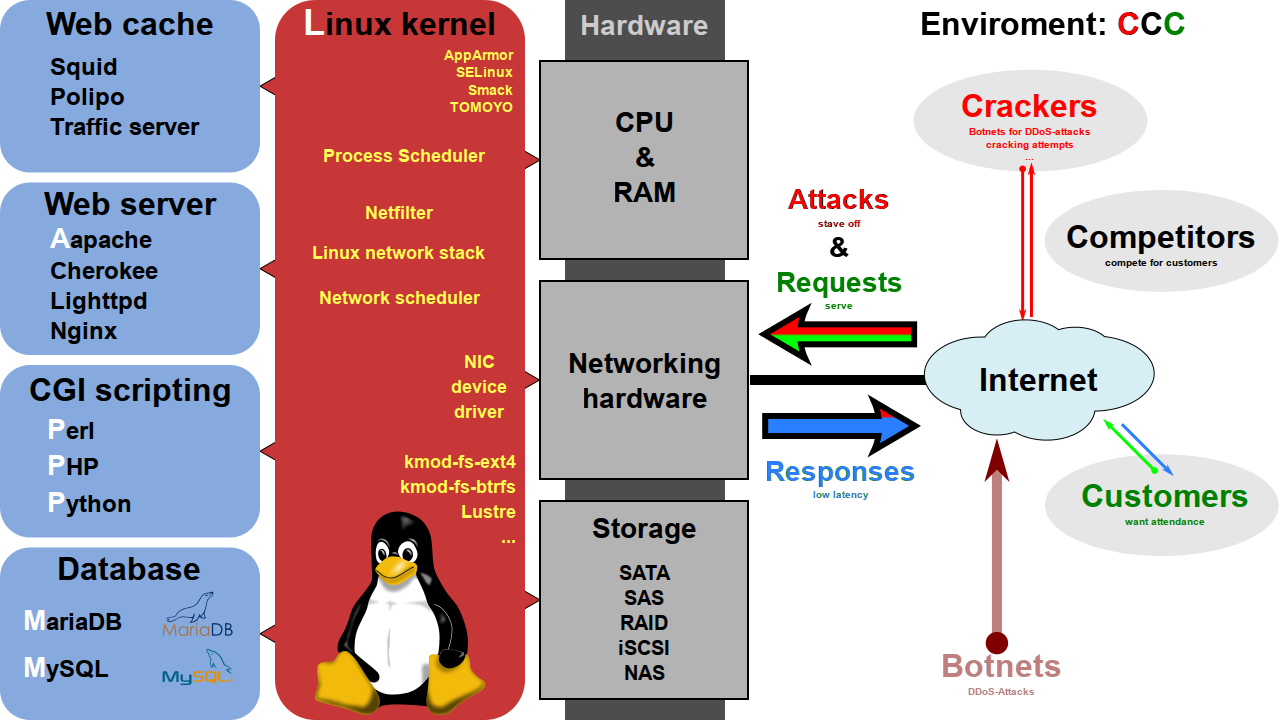
\includegraphics[scale=0.3]{LAMP_software_bundle.png}
\caption{The LAMP Architecture}
\label{LAMP_software_bundle}
\end{figure}

Broad overview of the LAMP software bundle, displayed here together with Squid. A high-performance and high-availability web server solution providing security in a hostile environment.

As of April 2007, over 20 million Internet domains had web services hosted on servers with PHP installed and \textcolor{Blue}{\texttt{mod\_php}} was recorded as the most popular Apache HTTP Server module.[94] PHP is used as the server-side programming language on 75\% of all websites whose server-side programming language is known, and PHP is the most-used open source software within enterprises. Web content management systems written in PHP include MediaWiki, Joomla, eZ Publish, SilverStripe, WordPress, Drupal, Moodle, the user-facing portion of Facebook, and Digg.

For specific and more advanced usage scenarios, PHP offers a well defined and documented way for writing custom extensions in C or C++. Besides extending the language itself in form of additional libraries, extensions are providing a way for improving execution speed where it is critical and there is room for improvements by using a true compiled language. PHP also offers well defined ways for embedding itself into other software projects. That way PHP can be easily used as an internal scripting language for another project, also providing tight interfacing with the project's specific internal data structures.


\section{Frameworks}

PHP官方的框架为Zend framework,2005年开始开发至今已经步入成熟期,尽管对于PHP框架的方向业界还有争议,但在实际生产中框架的使用已非常普遍。

另一些常用的PHP框架有:Yii、CodeIgniter、CakePHP、Symfony、QeePHP/FleaPHP、ThinkPHP等,使用这些框架,可以使项目得到更快更简单的部署和更加敏捷的开发效率,但在另一方面,学习这些框架的使用需要付出额外的学习成本。





\section{Libraries}



内置多样化的函数是PHP主要的特点之一,这些开放代码的函数提供了各种不同的功能,例如文件处理、FTP、字符串处理、等等。这些函数的使用方法和C语言相近(例如printf),这也是PHP广为流行的原因之一。

除了内置的函数之外,PHP也提供了很多扩展库(extension),像是各种数据库连接函数、数据压缩函数、图形处理等等。有些延伸库需要从PECL(PHP Extension Community Library)取得。

以下是PHP编程语言提供的库列表。



\begin{table}
\centering
\caption{PHP Libraries}
\label{php_libraries}
\rowcolors{1}{White}{Lavender}
\begin{tabular}{m{65pt}m{135pt}m{90pt}m{80pt}}
Apache			&Gettext						&mSQL			&SESAM\\
BCMath			&GD Graphics Library			&MySQL		&Session Handling\\
Bzip2			&GNU Multi-Precision Library	&Mowhawk		&Shared memory\\
Calendars		&Hyperwave					&muscat		&SMTP\\
CCVS			&iconv							&Ncurses		&SNMP\\
COM			&IMAP,POP3 and NNTP		&ODBC			&Sockets\\
ClibPDF			&Informix						&Oracle		&SimpleXML\\
cURL			&Ingres II						&OpenSSL		&SQLite\\
Cybercash		&InterBase						&Ovrimos SQL	&Streams\\
DB2			&IRC							&PDF			&Sybase\\
dBase			&LDAP							&PayFlow Pro	&Token\\
DBM			&Lotus Notes					&PDO			&vpopmail\\
dbx				&mailparse						&POSIX			&WDDX\\
DB++			& MCAL							&PostgreSQL	&Win32 API\\
DOM XML		&Mcrypt						&Printer		&XML(Xpath)\\
.NET			&MCVE							&Pspell			&XML-RPC\\
FileMaker Pro	&Mhash							&GNU Readline	&XSLT\\
FrontBase		&MIME Functions				&GNU Recode	&YAZ\\
filePro			& MS-SQL						&Regular expressions&Yellow Pages/NIS\\
FriBiDi			&Ming							&QT-Dom		&ZIP\\
FTP				&mnoGoSearch					&Semaphores	&Zlib\\


\end{tabular}
\end{table}




\chapter{Security}


About 30\% of all vulnerabilities listed on the National Vulnerability Database are linked to PHP. These vulnerabilities are caused mostly by not following best-practice programming rules. Technical security flaws of the language itself or of its core libraries are not frequent (23 in 2008, about 1\% of the total). Recognizing that programmers make mistakes, some languages include taint checking to automatically detect the lack of input validation which induces many issues. Such a feature is being developed for PHP, but its inclusion in a release has been rejected several times in the past.

There are advanced protection patches such as Suhosin and Hardening-Patch, especially designed for web hosting environments.

Some of the vulnerabilities are induced by improper PHP's runtime configuration. For example, failing to disable PHP execution for the directory where uploaded images are stored, can result in execution of malicious PHP code embedded within uploaded images. Another well known example is leaving enabled the dynamic loading of PHP extensions, in a shared hosting environment.










\chapter{Criticism}




PHP has been criticized for its heavy cluttering of main distribution with many functions, case-insensitive function names, among other specific details.


PHP has also been criticized heavily for the security vulnerabilities that can be created by certain language features, induced by some of the historically default values for their associated runtime settings. Among these, magic quotes and \textcolor{Blue}{\texttt{register\_globals}} are the best known. The latter made any URL parameters become variables, which while making programming easier, could create serious security vulnerabilities as it allowed an attacker to set the value of any variable and interfere with script execution.

It is felt PHP interferes with productivity because the lack of language design introduces unpredictable behavior, inconsistent function naming and parameter usage, dependency on new constructs to work around lower level language quirks, introduction of new constructs with flaky behavior, and missing or inconsistent error handling features.


It also lacks features such as native Unicode support and multithreading at the PHP core level, though using threads is made possible by the pthreads PECL extension.



















































































